
\chapter{Aufgabe D12}
Füllt der Fahrer seine Reifen wieder auf ist es unwahrscheinlich, dass alle Reifen den exakt gleichen Druck haben. Deswegen wird eine Resetfunktionalität implementiert, die diese Ungenauigkeiten in der Berechnung für Reifendruckabfälle mit einbezieht.\\ 
Dieser Reset soll vom Fahrer manuell betätigt werden und kann nur initiiert werden, wenn das Fahrzeug steht. Dafür wird das folgende Modul in \autoref{fig:Reset} verwendet.
\begin{figure}[H]
	\centering
	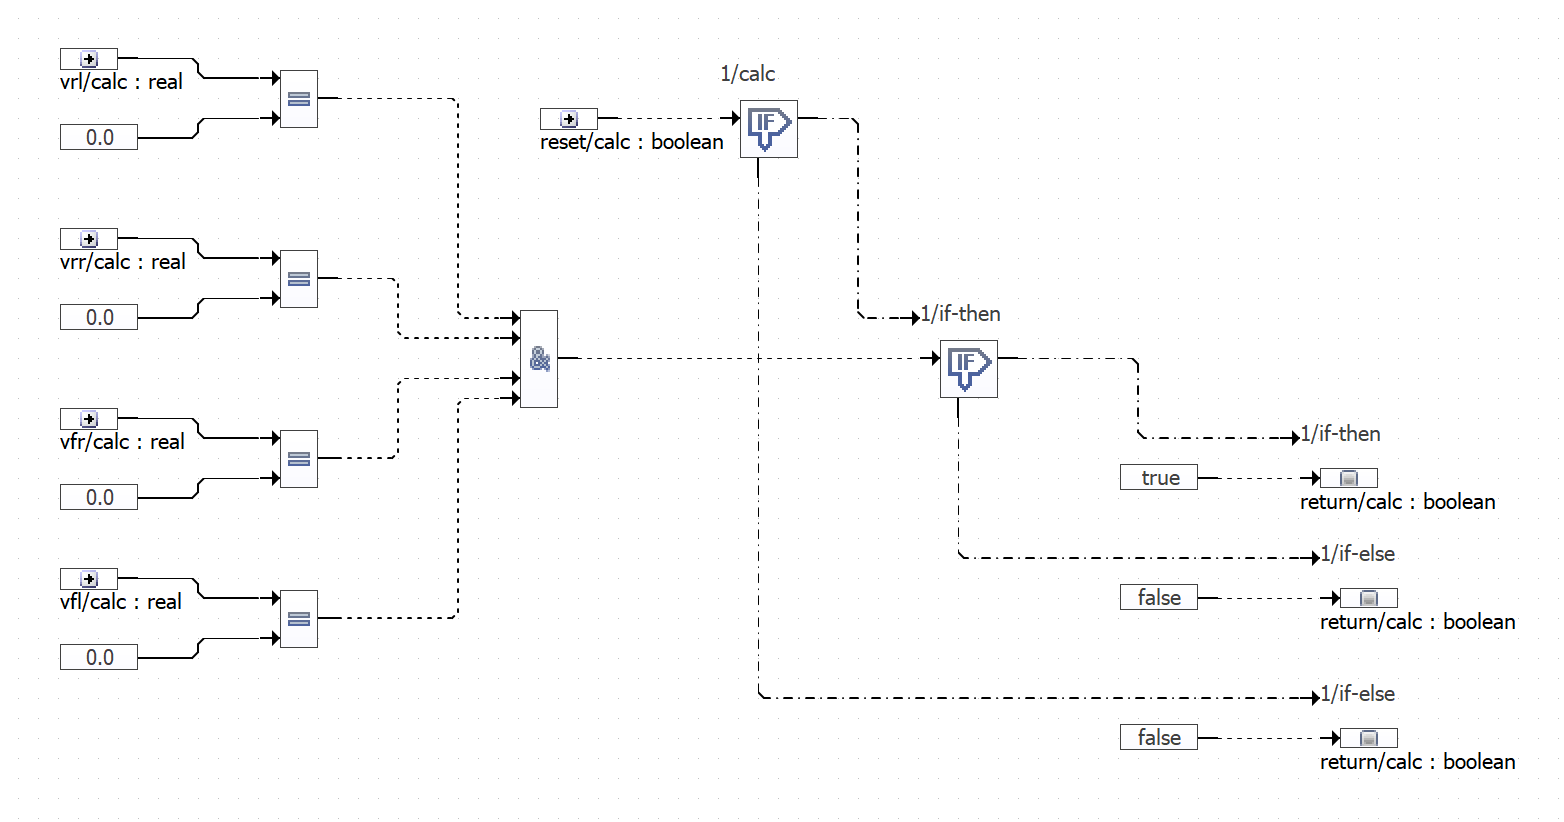
\includegraphics[width=0.9\linewidth]{../Graphiken/Reset.png}
	\caption{Reset Funktion}
	\label{fig:Reset}
\end{figure}
Eine Ebene höher interagiert die Funktion mit einer Statemachine die den Reset bearbeitet.
 \begin{figure}[H]
 	\centering
 	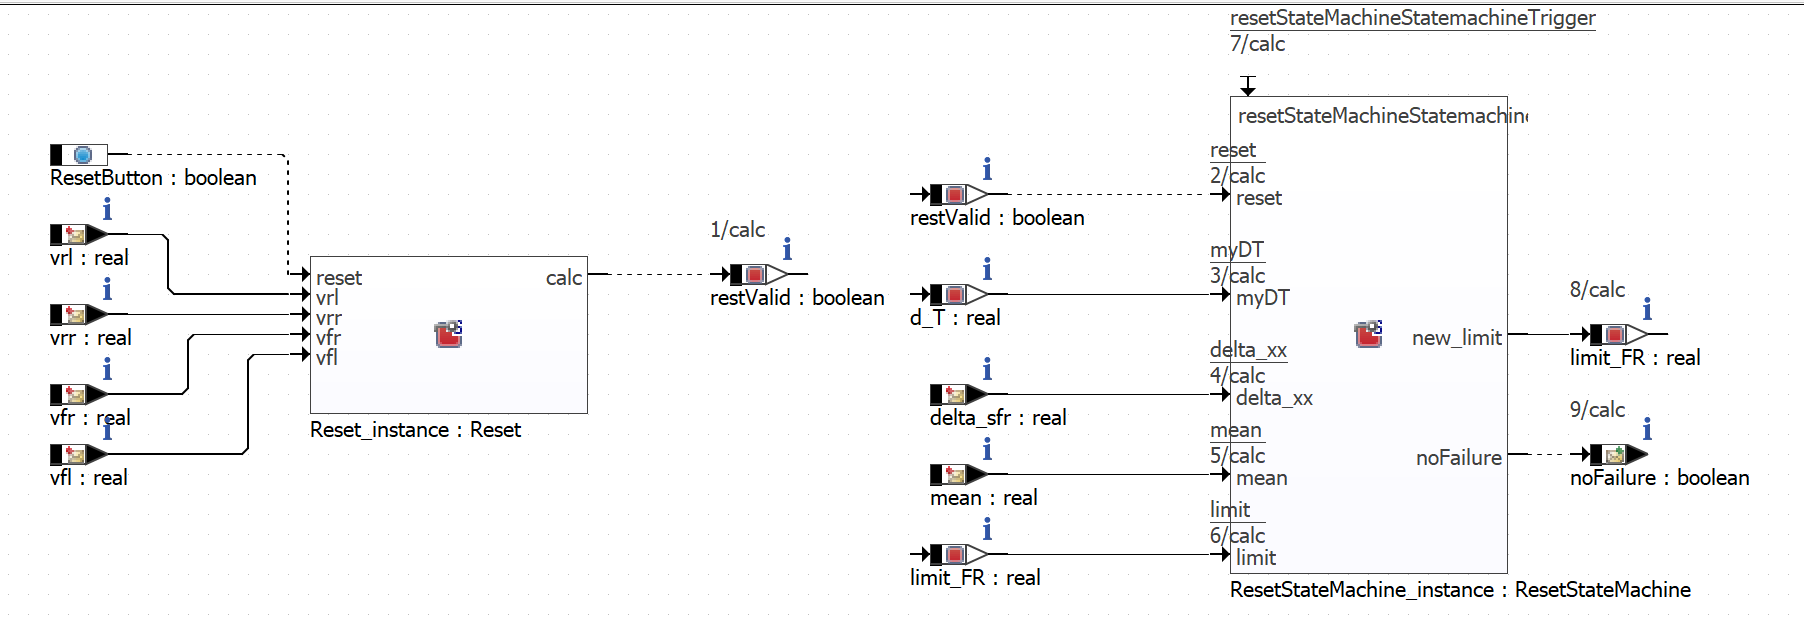
\includegraphics[width=\linewidth]{../Graphiken/ResetTop1.png}
 	\caption{Reset}
 	\label{fig:ResetTop}
 \end{figure}

Die Statemachine ist vierfach für jeden Reifen ausgeführt. Sie besitzt als Inputs, ob der Reset valid ist, das dT, das Streckendelta eines Reifens, den Durchschnitt aller Reifen, sowie das Limit bei dem ein Failure erkannt wird. Als Output gibt die Statemachine das neue Limit sowie eine Message an, die das Signalisieren eines zu hohen oder zu niedrigen Reifendurcks unterdrücken kann.\\
Die Reset-Statemachine besitzt vier States.
\begin{figure}[H]
	\centering
	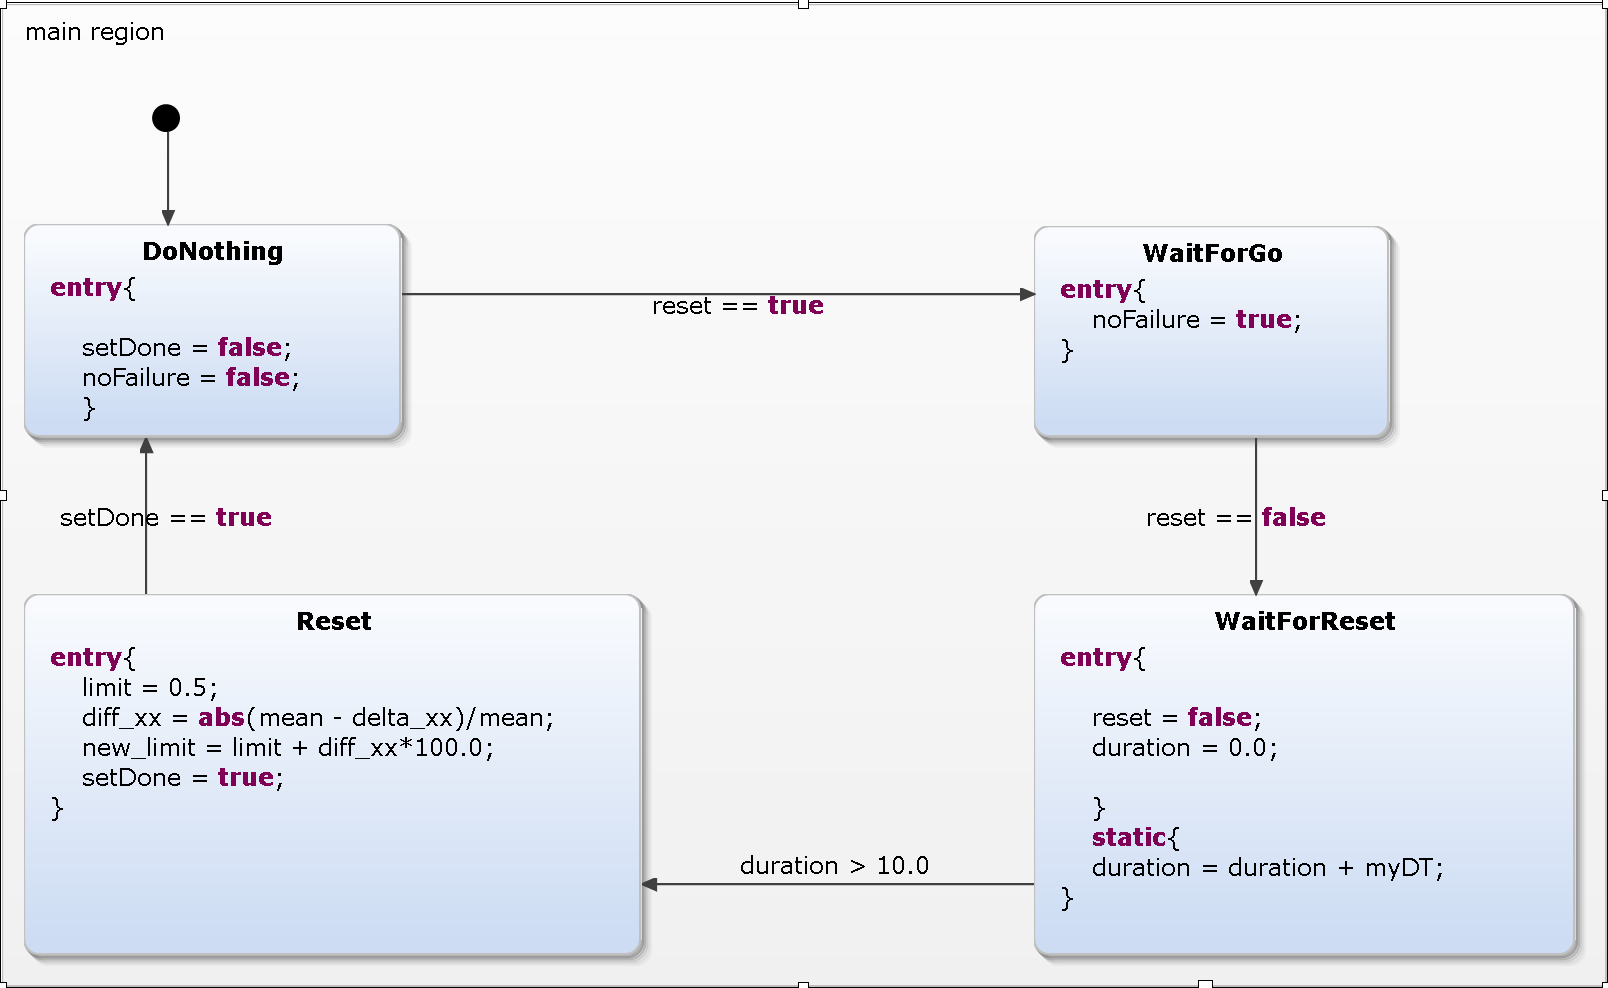
\includegraphics[width=1\linewidth]{../Graphiken/ResetStateMachine.png}
	\caption{Reset Statemachine}
	\label{fig:ResetStateMachine}
\end{figure}
Im DoNothing-State befindet sich die Statemachine solange die Reset-Taste nicht gedrückt bzw. der Reset nicht akzeptiert wurde. Liegt ein valider Reset vor wechselt die Statemachine in WaitForGo. Ab diesem State werden vorerst alle Reifenfehlermeldungen unterdrückt, da während einem Reset ja kein Fehler auftauchen soll. Fährt das Auto los, beginnt der eigentliche Reset des Systems. Durch das Losfahren ist der Reset-Parameter nicht mehr aktiv und die Statemachine wechselt in den State WaitForReset. In diesem State wartet das System, bis es sich sich eingeschwungen hat, sodass Noise das System nicht verfälscht. Ab einer gewissen Zeit wechselt die Statemachine in den Reset-Zustand. In diesem wird nun, wie auch in \autoref{fig:devCalc}, die momentane prozentuale Abweichung berechnet und auf das Standardlimit addiert. Dadurch wird die Abweichung für diesen Reifen um soviel größer, wie der Reifendruck momentan abweicht. Weicht der Reifendruck dann von dem neu kalibrierten Wert wieder 0.5\% ab, wird wieder ein Failure erkannt. Nach dem erfolgreichen Reset wechselt die Statemachine in DoNothing, wo auch wieder das Erkennen von Reifendruckabfällen freigeschaltet wird.\\
Dieser Reset wird parallel in drei weiteren Statemachines für die anderen Reifen durchgeführt.\\

Um dies im Environment zu testen, wird vor Start mit Hilfe des Error-Moduls, der Reifendruck der Reifen manipuliert und der Reset aktiviert.
Neue Limits werden nach dem Losfahren des Fahrzeugs generiert.
\begin{figure}[H]
	\centering
	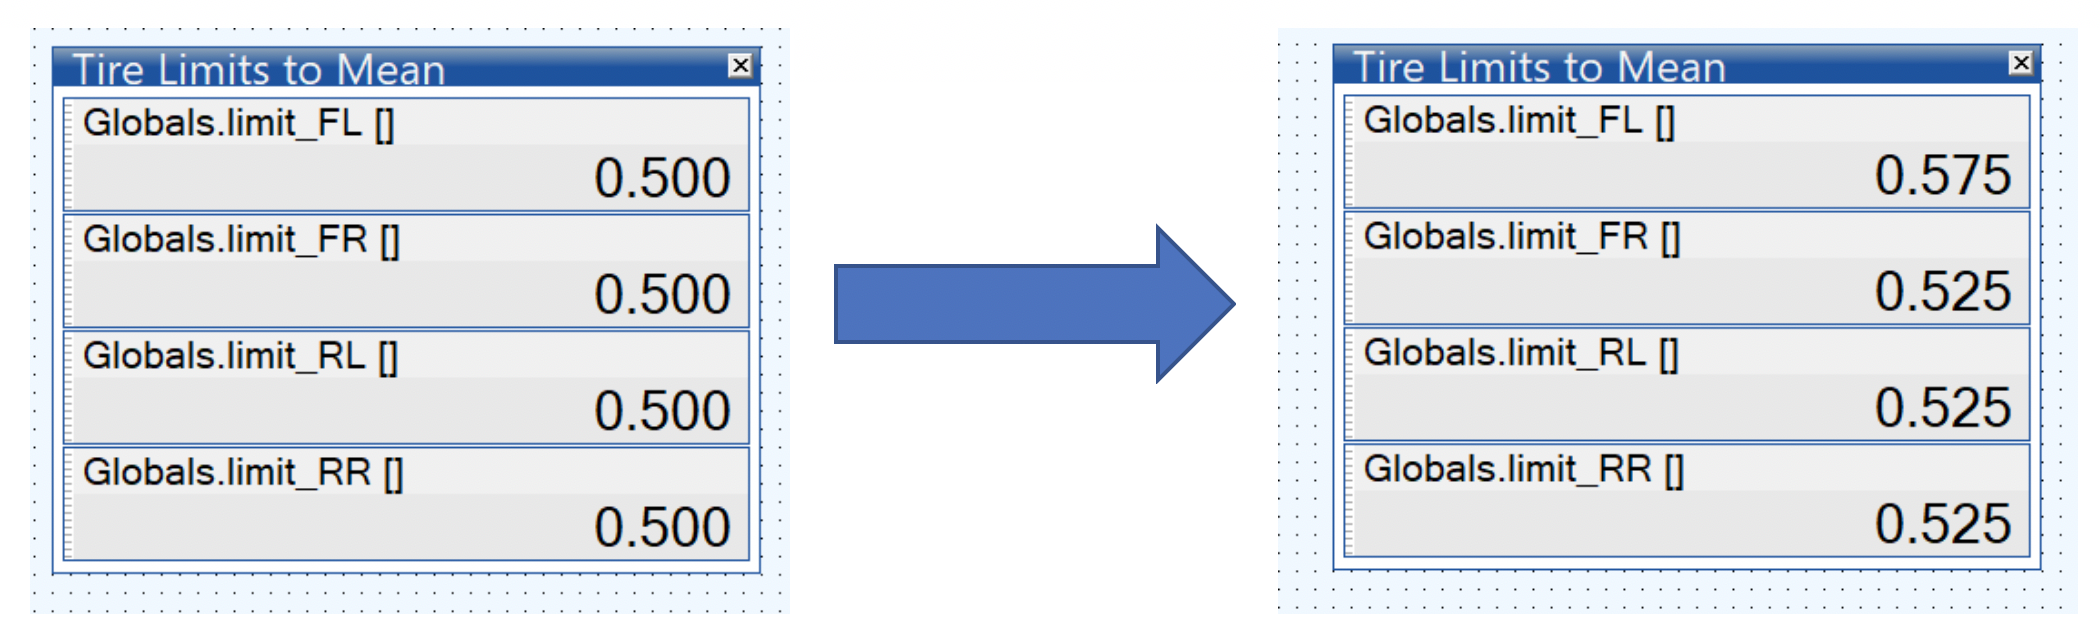
\includegraphics[width=1\linewidth]{../Graphiken/ResetDone.png}
	\caption{Neue Limits nach Reset}
	\label{fig:ResetState}
\end{figure}
Die neuen Limits sind keineswegs größer. In ihnen ist nur schon die Abweichung der Reifen zum Normalzustand miteinberechnet, sodass sich bei der Berechnung nichts ändert.